\documentclass[11pt,a4paper]{article}
\usepackage[margin=23mm]{geometry}
\usepackage[T1]{fontenc}
\usepackage{lmodern}
\usepackage{graphicx,booktabs,longtable,amsmath,array,xcolor}
\usepackage[hidelinks]{hyperref}
\graphicspath{{figures/}}
\setlength{\parindent}{0pt}
\setlength{\parskip}{5pt}
\setlength{\emergencystretch}{2em}
\renewcommand{\arraystretch}{1.15}
\title{RankWalk: Paper Reproduction and Expanded Longitudinal Evaluation}
\author{Computational evaluation report}
\date{9 November 2026}
\begin{document}
\maketitle
\begin{abstract}
This report reruns the RankWalk paper experiments using the corrected CPU-accelerated implementation, reproduces four original clinical cohorts, and extends the comparison to six longitudinal cohorts and additional representation methods. Repository settings are the primary specification; paper-specification sensitivities and compatibility corrections are identified separately. All 300 RankWalk simulation fits and all 90 original clinical fits completed. Three VaDER fits failed numerical checks despite retries. RankWalk is competitive but does not dominate all settings: TS2Vec leads the regime-switching simulation, and simple summaries or TimesURL outperform the common RankWalk configuration on PAQUID. Strong visit-time-only controls show that full-follow-up clinical concordance must be interpreted as descriptive association, not prospective prediction.
\end{abstract}
\tableofcontents
\clearpage
\section{Scope, completion, and statistical interpretation}
The reference is the uploaded paper \emph{Contrastive Representation Learning of Longitudinal Disease Trajectories on Temporal Graphs}, arXiv:2607.25609. The software checkout is RankWalk commit \texttt{58a87af4fdcdd243425106622e0e4f46dcc1ba6a}. This evaluation changed no tracked repository files and pushed nothing.

The design comprises six RankWalk simulation settings with 50 repetitions each; 20 PBC2, 20 AIDS, 20 HEART, and 30 PAQUID original-protocol clinical fits; and ten requested fits per extension method and cohort. Numerical failures are reported, not replaced by selected seeds or fabricated scores. The strict all-successful flag in the provenance audit remains false because of the three failed VaDER fits, although the compute queue has finished.

Simulation accuracy is measured by adjusted Rand index (ARI), with known cluster labels used only for evaluation. Clinical outcomes are summarized by concordance and log-rank chi-square after clustering full observed trajectories. Cluster risk ordering uses observed follow-up times, except the native PAQUID script, which uses a fitted categorical Cox model. These are in-sample, post-hoc association measures. They are not held-out predictive accuracy or AUROC.

Every $\pm$ value is the sample standard deviation across repeated simulation datasets or stochastic fits. Clinical repeats reuse the same patients; their SD is algorithmic variation, not patient-sampling uncertainty. A reported SD of zero means identical repeated results, not absence of uncertainty. No exhaustive competitor hyperparameter search was performed.

\section{Methods and fixed budgets}
Simulations use 200 subjects, four balanced clusters, and five outcomes. Replicate seeds are 10001--10050. Compared methods receive the same generated dataset for each scenario and replicate. RankWalk uses sparse Jaccard similarity and the CPU Numba backend: 100 epochs, Adam learning rate $10^{-3}$, walk length 20, top-$k$ 10, and similarity-neighbor count 5. Regular-series node embeddings are flattened per subject, standardized, and clustered with R k-means using 50 starts.

Native R baselines are retained: B-spline FPCA with five basis functions and two components per marker; DTW distances with PAM; kml3d with ten redrawings; and TAPIO with 500 trees, four levels, and PC1 or variance-weighted PCA selection. Official TS2Vec uses 50 epochs and 64 output dimensions. Official VaDER uses hidden/latent dimensions [12,2], 50 pretraining plus 100 fitting epochs, batch size 64, and its native Gaussian-mixture clusters for simulation ARI.

Real-data extensions additionally include TimesURL (200 updates, 64 output dimensions), simple marker summaries, and visit-time/count controls. Sequence encoders receive a common 32-point absolute-time interpolation with global marker standardization; FPCA uses native sparse PACE; RankWalk uses the observed graph, mean pooling, 100 epochs, walk length 20, top-$k$ 10, five similarity neighbors, and grid overlap 0.5. Standardized representations feed k-means with 100 starts. VaDER is shown both with native mixture assignments and with posterior embeddings followed by common k-means; these are different readouts of the same fitted model, not independent fits.

Visit-time controls contain minimum, maximum, mean, SD, range, and count of observed visit times. Marker summaries contain mean, SD, first and last value, and slope per marker. These unsupervised controls require no outcome labels during representation construction. They expose association carried by the observation process or simple trajectory summaries.

The new cohorts are PROTHRO (488 cirrhosis-trial patients) and RENAL (407 renal-transplant patients). RENAL has over 180,000 marker records; data are aggregated into 32 prespecified absolute-time bins, with GFR log-transformed, before the graph/FPCA comparison. Original cohort sources are public JM, joineR, and joineRML package data. Source commits and package versions accompany this report.

\section{Specification differences and explicit corrections}
\begin{enumerate}
\item \textbf{Simulation 1 random curves.} The repository redraws quadratic random-curve coefficients per visit. The paper describes one curve per subject. The repository version is primary; the subject-shared version is a separate sensitivity. Clean noise uses marker-effect SDs of 5. The noisy-marker condition starts at 3 and replaces one marker SD by an integer drawn from 3--20. Thus the clean and noisy panels differ in base noise; the noisy panel is not an isolated addition of noise to the clean panel.
\item \textbf{Irregular readout.} The source irregular script flattens unequal-length trajectories into incompatible rows. The evaluation interpolates node embeddings to a ten-point global absolute-time grid before flattening. Graph and readout settings differ between regular and irregular pipelines, so their difference cannot be attributed solely to sampling irregularity.
\item \textbf{TS2Vec serialization and latent state.} Simulation 1 source input is $N\times50\times2$ (long-format outcome identifier and value), rather than the observed-marker $N\times10\times5$ tensor. Both are reported. Simulation 2 adds latent regime state to the source TS2Vec input and to the R wide matrix used by other baselines. Observed-only inputs are the valid main comparison. Source-input leakage diagnostics are shown separately and cannot support an observed-data superiority claim.
\item \textbf{Clinical cluster counts.} Source scripts use $K=3$ for PBC2, AIDS and PAQUID and $K=2$ for HEART, whereas the paper text describes $K=4$. Source $K$ is primary; $K=4$ is a separate sensitivity. Actual source GNN calls use 100 epochs for PBC2/HEART/PAQUID and 200 for AIDS. Source HEART/PAQUID graph settings use ten neighbors, overlap 0.8, and walk/top-$k$ 5. HEART's common extension configuration therefore differs materially from its primary configuration.
\item \textbf{PAQUID endpoint and readout.} The subject-level eventual dementia indicator is treated as visit-specific in the source, assigning event time zero to dementia cases. That native result is retained only for reproduction. The extension uses \texttt{agedem} minus baseline age, excludes nonpositive times, and applies common Hmisc concordance. Native PAQUID uses zero-padded flattened embeddings; the common extension uses mean pooling. Correcting the endpoint on saved native representations is a different sensitivity from rerunning the common extension.
\item \textbf{Other compatibility details.} Source AIDS duplicates CD4 as two channels; primary reproduction preserves this and the extension removes duplication. Undefined standardized constant padding columns are set to zero. Primary clinical R clustering, Torch initialization and walk sampling are seeded, but the source clinical NumPy graph-subspace RNG was not pre-seeded. Saved representations permit exact metric replay, while graph refits retain that reproducibility limitation.
\end{enumerate}

\section{Simulation results}
\subsection{Primary regular-data comparison}


\begin{table}[htbp]
\centering\small
\caption{Mean ARI $\pm$ SD. All cells use 50 replicates except VaDER S2 (49 successful fits). Source-serialized TS2Vec is a separate input sensitivity; its leaked S2 version is excluded here.}
\begin{tabular}{lccc}\toprule
Method & S1 clean & S1 noisy marker & S2 switching \\ \midrule
RankWalk & $0.924 \pm 0.039$ & $0.936 \pm 0.100$ & $0.911 \pm 0.080$ \\
FPCA & $0.913 \pm 0.038$ & $0.644 \pm 0.294$ & $0.654 \pm 0.021$ \\
DTW & $0.888 \pm 0.047$ & $0.681 \pm 0.246$ & $0.839 \pm 0.068$ \\
kml3d & $0.888 \pm 0.043$ & $0.869 \pm 0.136$ & $0.659 \pm 0.021$ \\
TAPIO PC1 & $0.666 \pm 0.094$ & $0.820 \pm 0.169$ & $0.676 \pm 0.032$ \\
TAPIO weighted & $0.811 \pm 0.082$ & $0.938 \pm 0.092$ & $0.681 \pm 0.033$ \\
TS2Vec (observed wide) & $0.573 \pm 0.177$ & $0.642 \pm 0.227$ & $0.961 \pm 0.053$ \\
TS2Vec (source serialization) & $0.770 \pm 0.077$ & $0.684 \pm 0.213$ & -- \\
VaDER (posterior + k-means) & $0.520 \pm 0.156$ & $0.563 \pm 0.215$ & $0.660 \pm 0.035$ \\
\bottomrule\end{tabular}
\end{table}

RankWalk has a small clean-setting advantage over FPCA. Under marker corruption it is essentially tied with weighted TAPIO. TS2Vec with observed-marker input leads Simulation 2. These findings do not support universal superiority of RankWalk. The unusually higher noisy-setting mean for some methods is not evidence that adding noise helps: the two panels use different base-noise settings.

\begin{table}[htbp]
\centering\small
\caption{Paired RankWalk minus comparator differences. Percentile bootstrap over 50 paired replicates, 10,000 resamples; exploratory intervals are not adjusted for multiple comparisons.}
\begin{tabular}{lccc}\toprule
Setting & Comparator & Mean $\Delta$ ARI & 95\% bootstrap interval \\ \midrule
S1 clean & FPCA & +0.011 & [+0.003, +0.019] \\
S1 clean & TAPIO weighted & +0.113 & [+0.095, +0.132] \\
S1 clean & TS2Vec (observed wide) & +0.350 & [+0.302, +0.398] \\
S1 noisy & FPCA & +0.292 & [+0.221, +0.361] \\
S1 noisy & TAPIO weighted & -0.003 & [-0.025, +0.018] \\
S1 noisy & TS2Vec (observed wide) & +0.294 & [+0.237, +0.348] \\
S2 & FPCA & +0.256 & [+0.235, +0.277] \\
S2 & TAPIO weighted & +0.230 & [+0.207, +0.251] \\
S2 & TS2Vec (observed wide) & -0.050 & [-0.068, -0.034] \\
\bottomrule\end{tabular}
\end{table}

\begin{figure}[htbp]\centering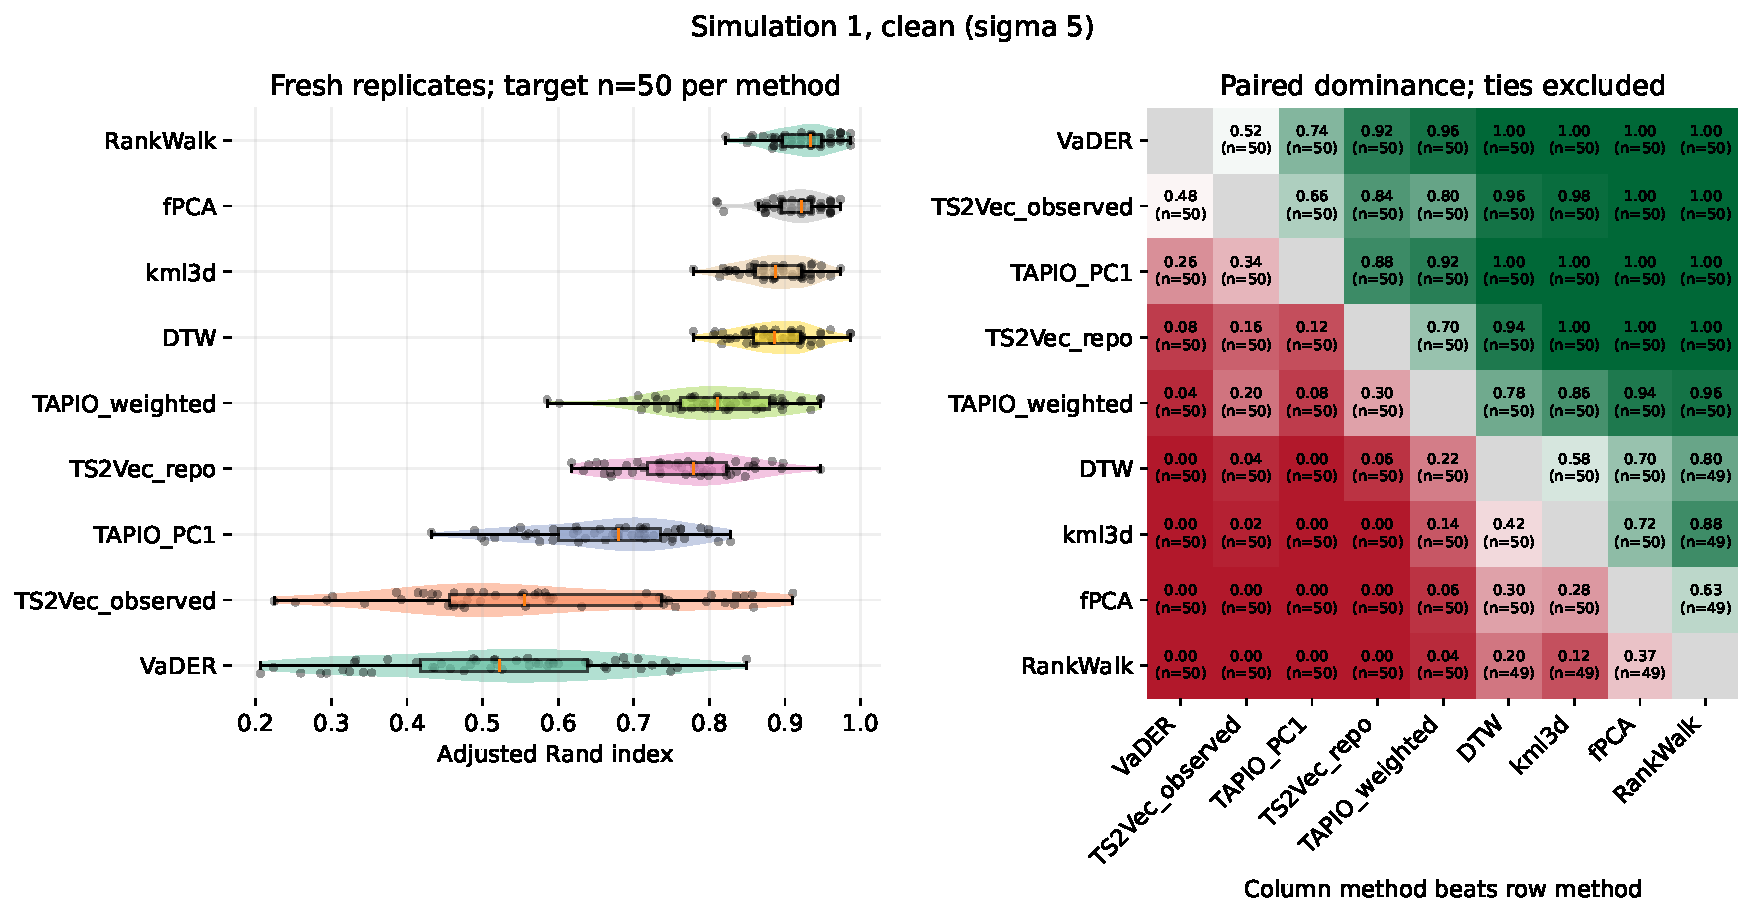
\includegraphics[width=\linewidth]{S1_clean.pdf}\caption{Clean Simulation 1. Horizontal violin/box/jitter plots and paired dominance heatmaps follow the reference paper style. A heatmap cell is the proportion of non-tied paired replicates in which the column method beats the row method; gray cells are undefined or diagonal. VaDER S2 comparisons use 49 available pairs.}\end{figure}

\begin{figure}[htbp]\centering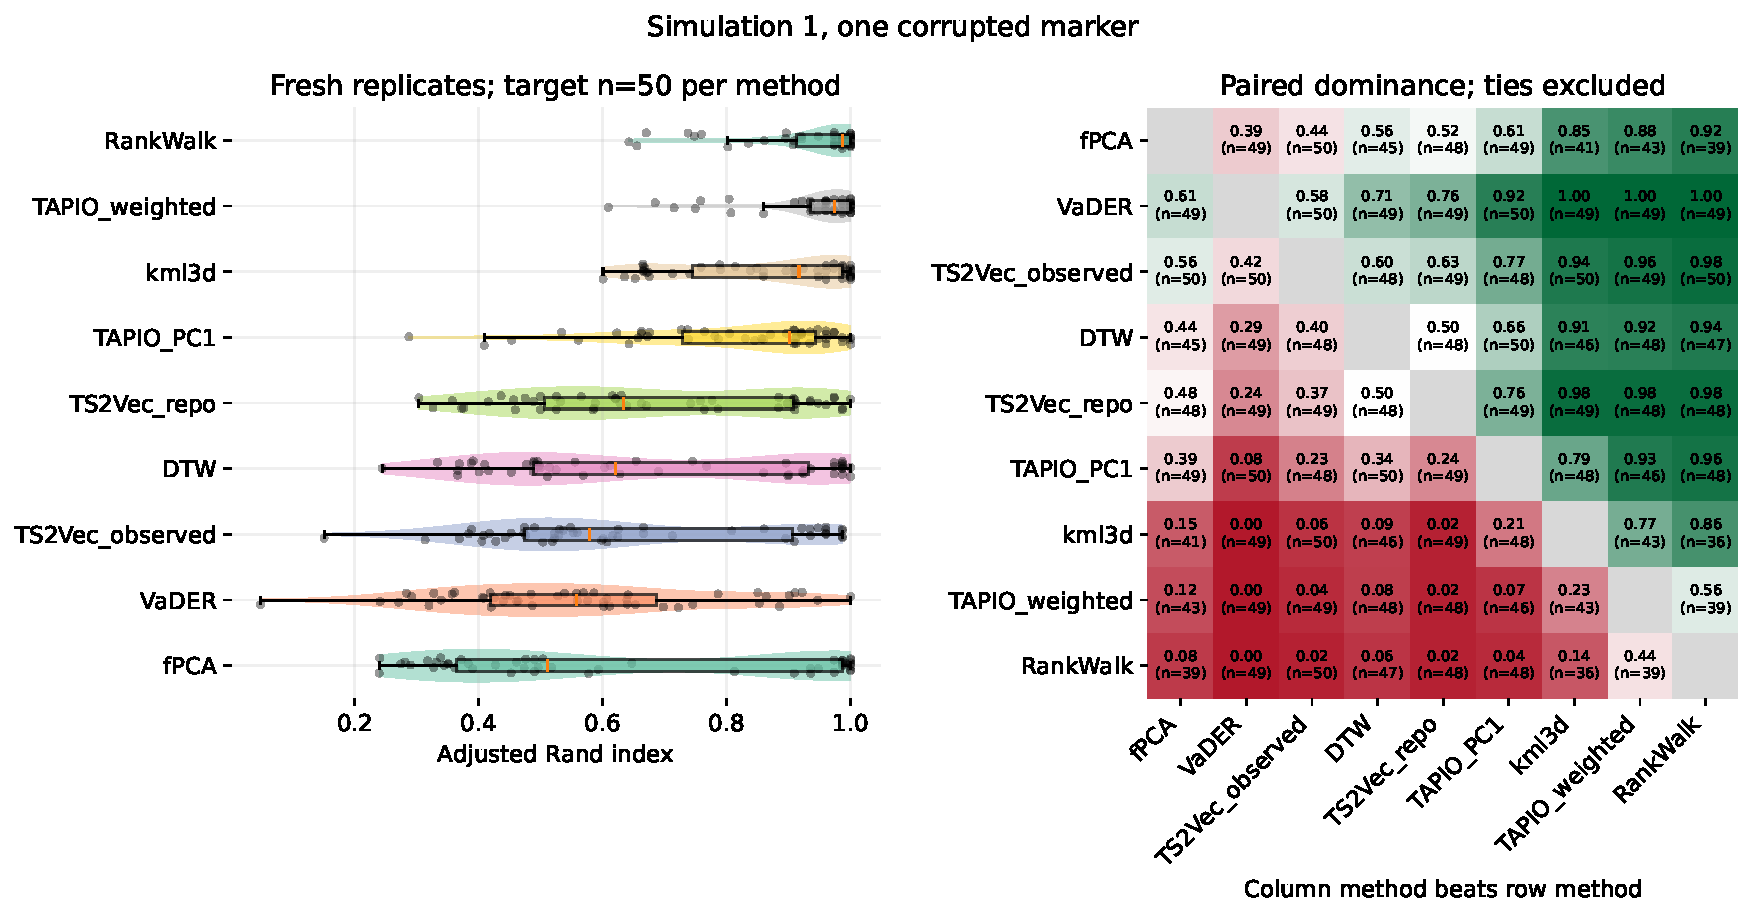
\includegraphics[width=\linewidth]{S1_noisy.pdf}\caption{Simulation 1 with one corrupted marker. Horizontal violin/box/jitter plots and paired dominance heatmaps follow the reference paper style. A heatmap cell is the proportion of non-tied paired replicates in which the column method beats the row method; gray cells are undefined or diagonal. VaDER S2 comparisons use 49 available pairs.}\end{figure}

\begin{figure}[htbp]\centering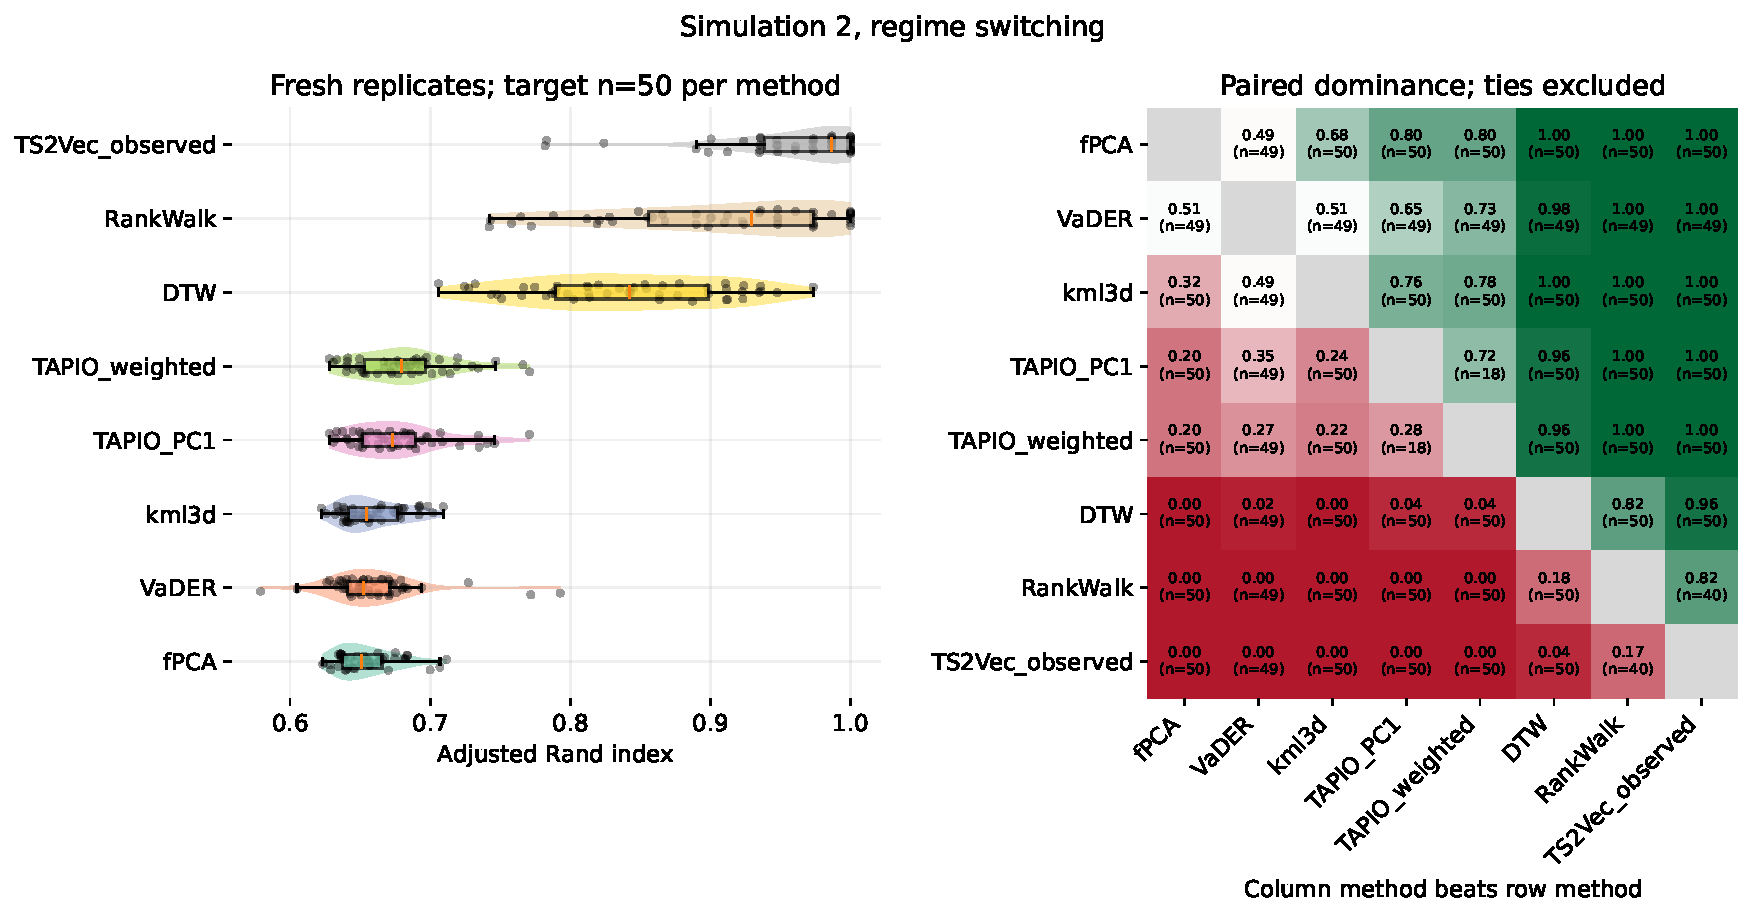
\includegraphics[width=\linewidth]{S2_regular.pdf}\caption{Observed-marker Simulation 2; latent regime is excluded from the comparator input. Horizontal violin/box/jitter plots and paired dominance heatmaps follow the reference paper style. A heatmap cell is the proportion of non-tied paired replicates in which the column method beats the row method; gray cells are undefined or diagonal. VaDER S2 comparisons use 49 available pairs.}\end{figure}

\clearpage\subsection{Irregular sampling and subject-shared random curves}

\begin{table}[htbp]
\centering\small
\caption{All 300 RankWalk fits: six settings with 50 repetitions each.}
\begin{tabular}{lcc}\toprule
RankWalk setting & Fits & ARI \\ \midrule
S1 regular & 50 & $0.924 \pm 0.039$ \\
S1 irregular & 50 & $0.905 \pm 0.043$ \\
S2 regular & 50 & $0.911 \pm 0.080$ \\
S2 irregular & 50 & $0.921 \pm 0.090$ \\
S1 subject-shared curve & 50 & $0.782 \pm 0.081$ \\
\bottomrule\end{tabular}
\end{table}

The subject-shared-curve sensitivity gives RankWalk $0.782\pm0.081$ and FPCA $0.756\pm0.070$, substantially below their repository-generator results. This is a material specification effect. High irregular-data scores show recovery under the corrected pipeline; they do not isolate the causal effect of sampling irregularity.

\begin{figure}[htbp]\centering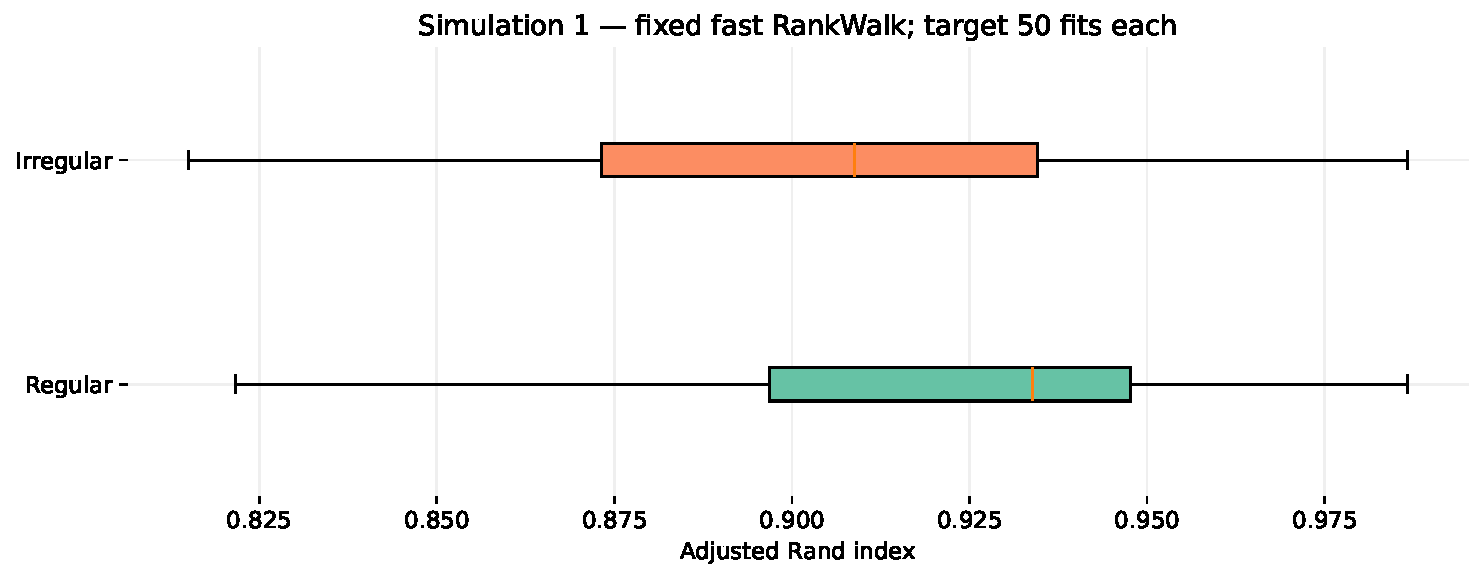
\includegraphics[width=\linewidth]{S1_clean_vs_irregular.pdf}\caption{Simulation 1, regular versus irregular RankWalk pipelines.}\end{figure}

\begin{figure}[htbp]\centering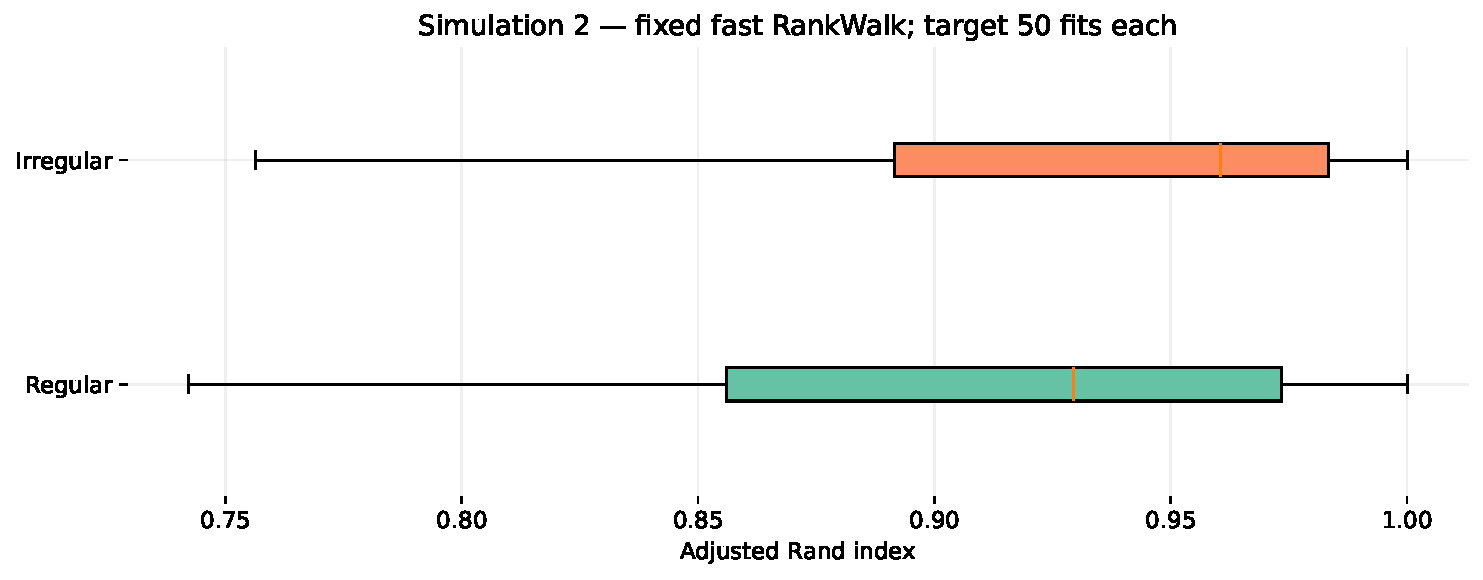
\includegraphics[width=\linewidth]{S2_regular_vs_irregular.pdf}\caption{Simulation 2, regular versus irregular RankWalk pipelines.}\end{figure}

\begin{figure}[htbp]\centering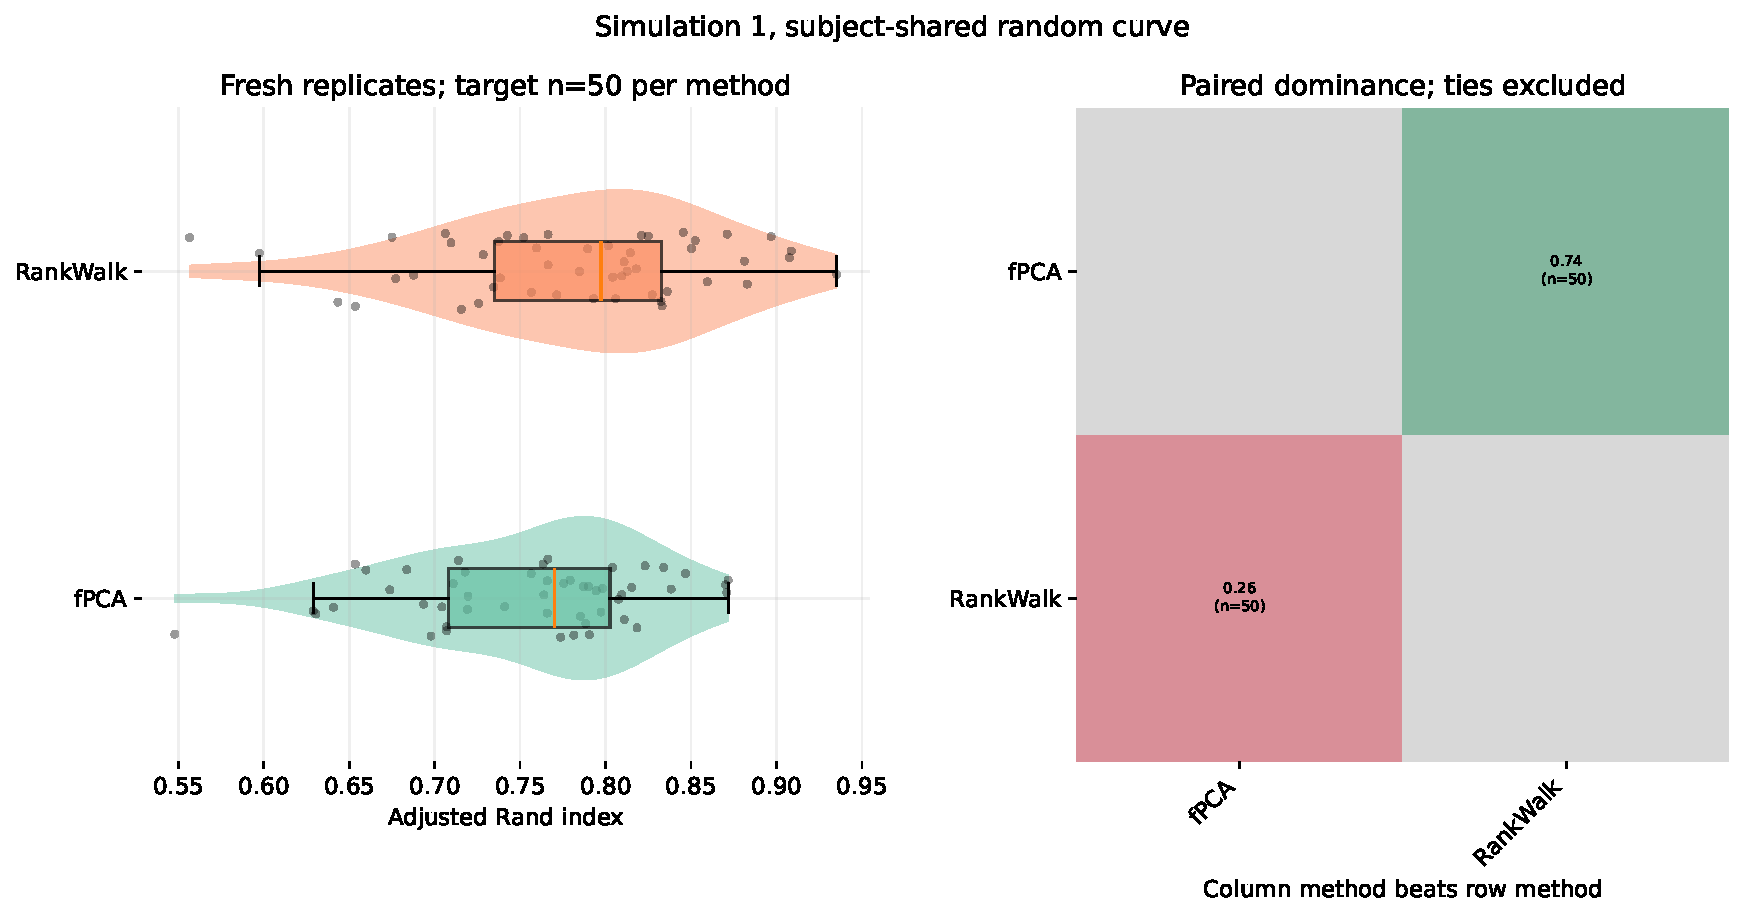
\includegraphics[width=\linewidth]{S1_subject_curve.pdf}\caption{Subject-shared random-curve sensitivity, compared with FPCA.}\end{figure}

\clearpage\section{Original clinical reproduction}

\begin{table}[htbp]
\centering\small
\caption{Completed primary clinical reproduction. Source cluster counts and readouts are preserved. Native PAQUID has a time-zero endpoint defect and Cox-derived concordance; it is not a valid incident-dementia prediction analysis.}
\begin{tabular}{lcccc}\toprule
Cohort & Method & Fits & C-index & Log-rank $\chi^2$ \\ \midrule
PBC2 & RankWalk & 20 & $0.788 \pm 0.018$ & $240.79 \pm 26.95$ \\
PBC2 & FPCA & 20 & $0.760 \pm 0.000$ & $127.50 \pm 0.00$ \\
AIDS & RankWalk & 20 & $0.689 \pm 0.006$ & $104.11 \pm 9.39$ \\
AIDS & FPCA & 20 & $0.642 \pm 0.000$ & $53.09 \pm 0.00$ \\
HEART & RankWalk & 20 & $0.706 \pm 0.022$ & $54.16 \pm 8.41$ \\
HEART & FPCA & 20 & $0.569 \pm 0.000$ & $4.81 \pm 0.00$ \\
PAQUID & RankWalk & 30 & $0.706 \pm 0.015$ & $40.20 \pm 5.05$ \\
PAQUID & FPCA & 30 & $0.659 \pm 0.000$ & $34.29 \pm 0.00$ \\
\bottomrule\end{tabular}
\end{table}

The fresh FPCA PBC2 values ($C=0.7603$, $\chi^2=127.50$), AIDS values ($0.6423$, $53.09$), and HEART values ($0.5693$, $4.81$) match the paper's rounded values. RankWalk means are also close to the reported values. PAQUID FPCA concordance matches the paper's rounded value, but the fresh source-script log-rank statistic is 34.29 versus the paper's 5.06. This discrepancy is retained rather than overwritten or assumed resolved.

\begin{figure}[htbp]\centering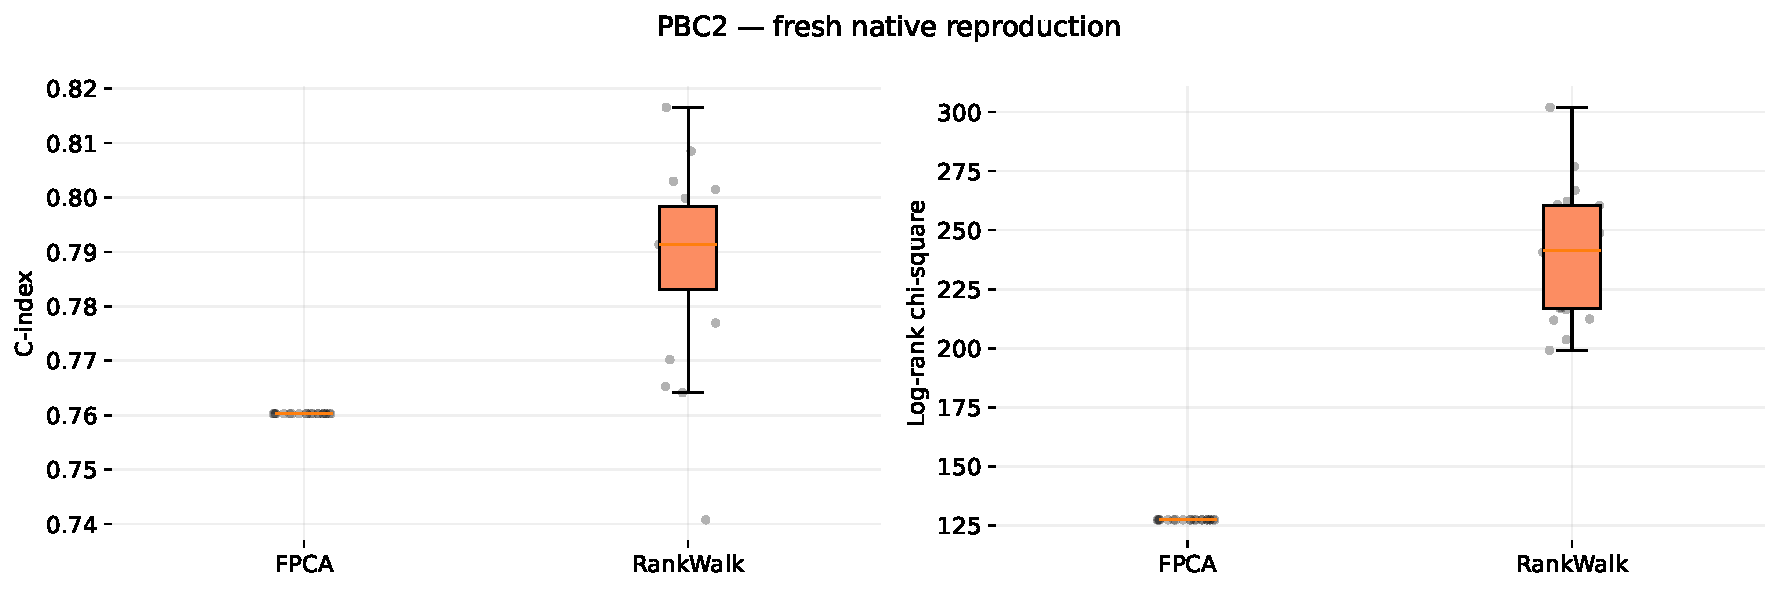
\includegraphics[width=\linewidth]{PBC2.pdf}\caption{PBC2 primary reproduction. Boxplots and jitter summarize repeated fits, not independent patient samples.}\end{figure}

\begin{figure}[htbp]\centering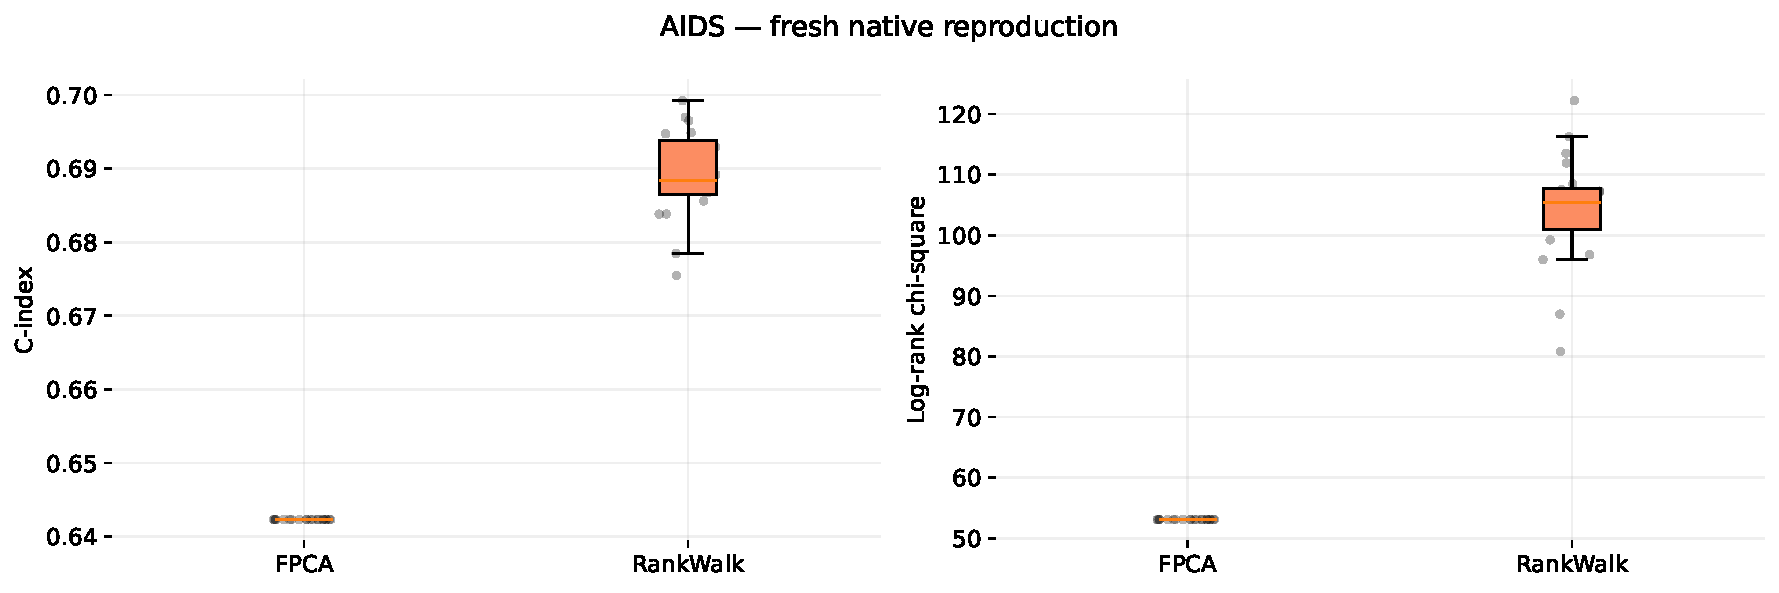
\includegraphics[width=\linewidth]{AIDS.pdf}\caption{AIDS primary reproduction. Boxplots and jitter summarize repeated fits, not independent patient samples.}\end{figure}

\begin{figure}[htbp]\centering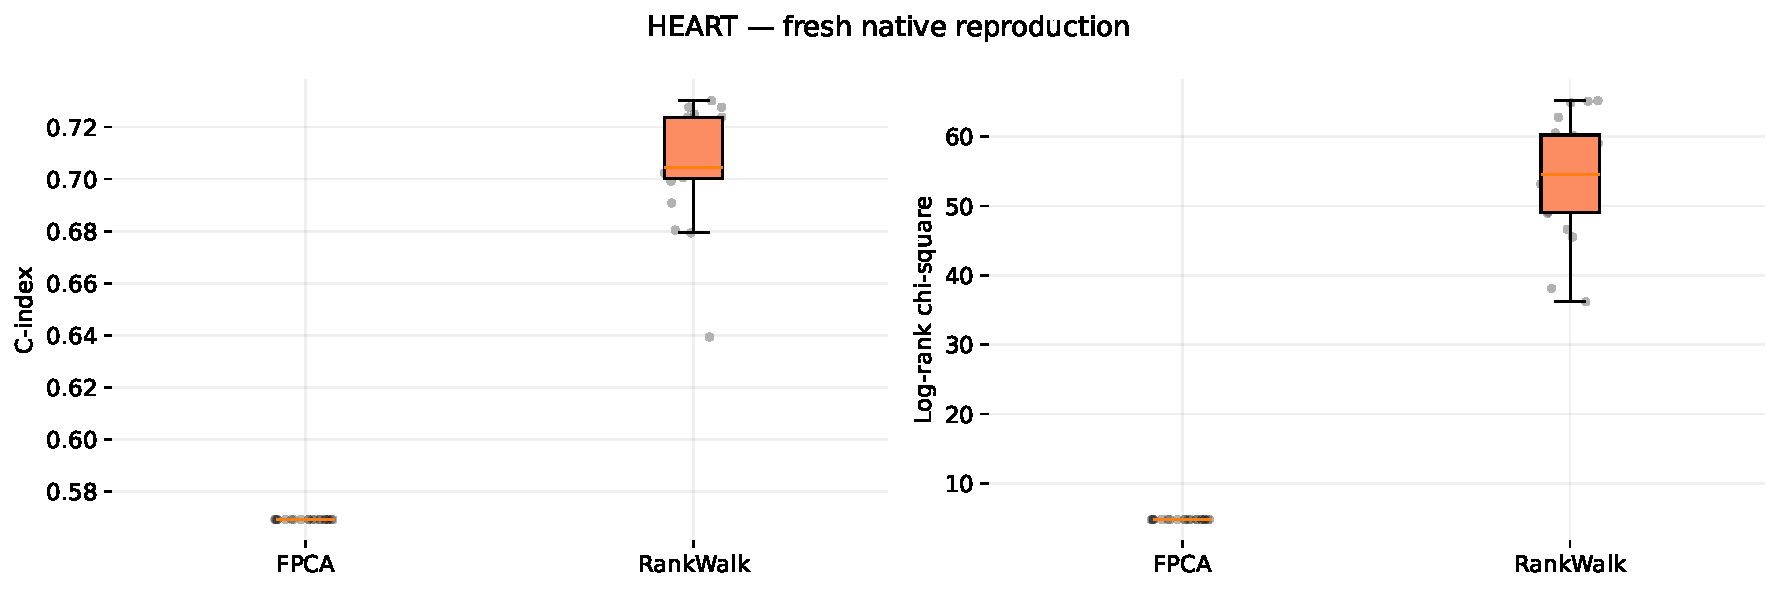
\includegraphics[width=\linewidth]{HEART.pdf}\caption{HEART primary reproduction. Boxplots and jitter summarize repeated fits, not independent patient samples.}\end{figure}

\begin{figure}[htbp]\centering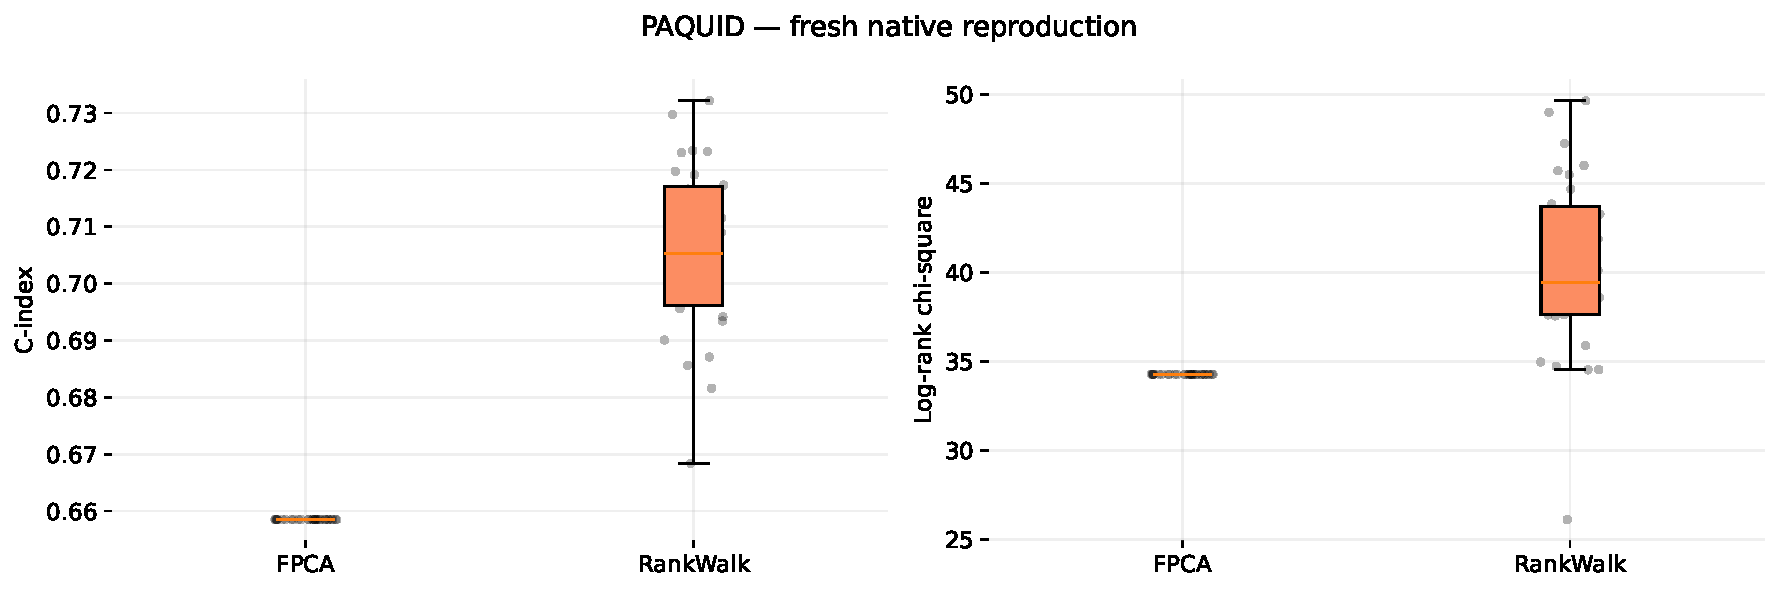
\includegraphics[width=\linewidth]{PAQUID.pdf}\caption{PAQUID primary reproduction. Boxplots and jitter summarize repeated fits, not independent patient samples.}\end{figure}

\clearpage\section{Expanded real-world comparison}

The following tables report successful fits on the common eligible cohort, using $K=3$ except HEART ($K=2$). Primary tables summarize each method's successful fits: VaDER has nine successes on RENAL and HEART, while the other methods have ten. Replicate-level data permit matched-subset comparisons; unequal-count means are not paired significance tests. Failure rates are reported separately. Zero SDs in deterministic controls indicate stable partitions on the same patients.

\begin{table}[htbp]
\centering\small
\caption{Mean C-index $\pm$ SD across successful extension fits. $\dagger$ denotes nine successful fits rather than ten. VaDER posterior and native-mixture rows are two readouts of the same model.}
\begin{tabular}{lccc}\toprule
Method & PBC2 & PAQUID & PROTHRO \\ \midrule
RankWalk & $0.788 \pm 0.027$ & $0.682 \pm 0.040$ & $0.707 \pm 0.010$ \\
FPCA & $0.760 \pm 0.000$ & $0.676 \pm 0.000$ & $0.636 \pm 0.000$ \\
TS2Vec & $0.656 \pm 0.057$ & $0.613 \pm 0.032$ & $0.668 \pm 0.034$ \\
TimesURL & $0.716 \pm 0.014$ & $0.746 \pm 0.022$ & $0.679 \pm 0.011$ \\
VaDER (native mixture) & $0.681 \pm 0.055$ & $0.638 \pm 0.089$ & $0.632 \pm 0.048$ \\
VaDER (posterior + k-means) & $0.711 \pm 0.014$ & $0.706 \pm 0.046$ & $0.657 \pm 0.024$ \\
Marker summaries & $0.729 \pm 0.001$ & $0.763 \pm 0.000$ & $0.637 \pm 0.000$ \\
Visit times/counts & $0.745 \pm 0.000$ & $0.682 \pm 0.000$ & $0.804 \pm 0.000$ \\
\bottomrule\end{tabular}
\end{table}

\begin{table}[htbp]
\centering\small
\caption{Mean C-index $\pm$ SD across successful extension fits. $\dagger$ denotes nine successful fits rather than ten. VaDER posterior and native-mixture rows are two readouts of the same model.}
\begin{tabular}{lccc}\toprule
Method & RENAL & AIDS & HEART \\ \midrule
RankWalk & $0.841 \pm 0.011$ & $0.689 \pm 0.009$ & $0.581 \pm 0.054$ \\
FPCA & $0.624 \pm 0.000$ & $0.642 \pm 0.000$ & $0.569 \pm 0.000$ \\
TS2Vec & $0.713 \pm 0.046$ & $0.526 \pm 0.037$ & $0.516 \pm 0.063$ \\
TimesURL & $0.741 \pm 0.017$ & $0.636 \pm 0.005$ & $0.521 \pm 0.065$ \\
VaDER (native mixture) & $0.719 \pm 0.055$$^{\dagger}$ & $0.617 \pm 0.018$ & $0.533 \pm 0.030$$^{\dagger}$ \\
VaDER (posterior + k-means) & $0.758 \pm 0.039$$^{\dagger}$ & $0.619 \pm 0.018$ & $0.535 \pm 0.060$$^{\dagger}$ \\
Marker summaries & $0.781 \pm 0.000$ & $0.641 \pm 0.000$ & $0.424 \pm 0.000$ \\
Visit times/counts & $0.887 \pm 0.000$ & $0.835 \pm 0.000$ & $0.705 \pm 0.000$ \\
\bottomrule\end{tabular}
\end{table}

\begin{table}[htbp]
\centering\small
\caption{Common extension-cohort sizes. PAQUID uses the corrected onset-age endpoint.}
\begin{tabular}{lccc}\toprule
Cohort & Primary extension $K$ & Subjects & Events \\ \midrule
PBC2 & 3 & 312 & 140 \\
PAQUID & 3 & 288 & 103 \\
PROTHRO & 3 & 488 & 292 \\
RENAL & 3 & 407 & 126 \\
AIDS & 3 & 467 & 188 \\
HEART & 2 & 256 & 54 \\
\bottomrule\end{tabular}
\end{table}

PBC2 favors RankWalk among these methods. PAQUID favors marker summaries and TimesURL; mean-pooled RankWalk is approximately comparable to FPCA. PROTHRO and RENAL favor RankWalk among biomarker representations but have even stronger visit-time/count controls. AIDS and HEART also show strong observation-process controls. Consequently, these metrics cannot establish biomarker-specific prognostic benefit or future clinical prediction.

HEART illustrates configuration sensitivity: the source-specific graph/walk configuration reproduces concordance near 0.706, whereas the common extension configuration is substantially weaker. PAQUID's extension also changes both readout and endpoint relative to the native source; its difference is not an isolated effect of faster training or endpoint correction.

\begin{figure}[htbp]\centering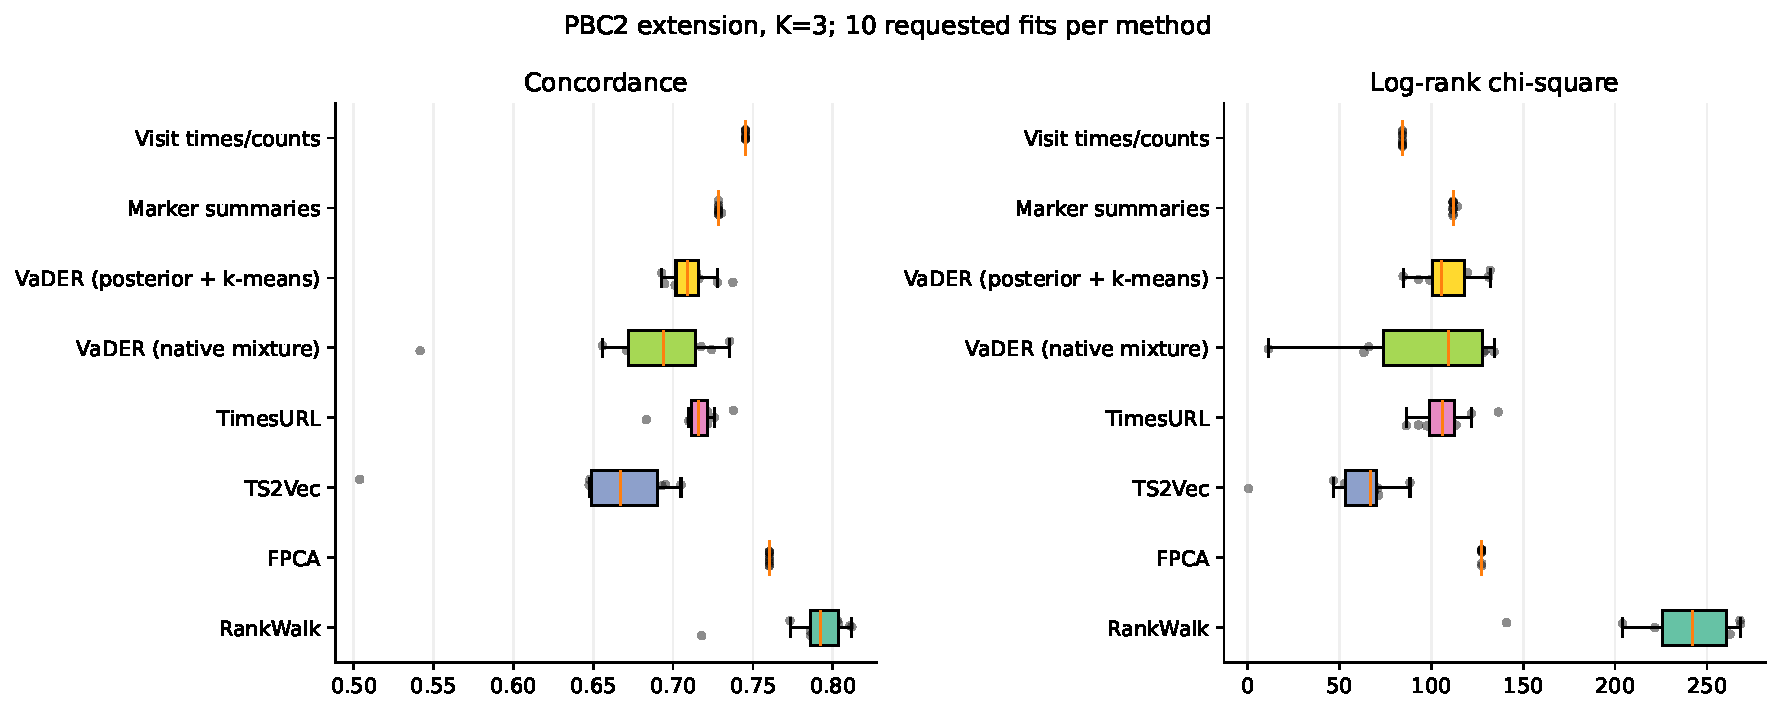
\includegraphics[width=\linewidth]{extension_PBC2.pdf}\caption{PBC2 final extension distributions. Nine native VaDER successes are shown for RENAL and HEART. The PAQUID endpoint is corrected; these are full-follow-up associations.}\end{figure}

\begin{figure}[htbp]\centering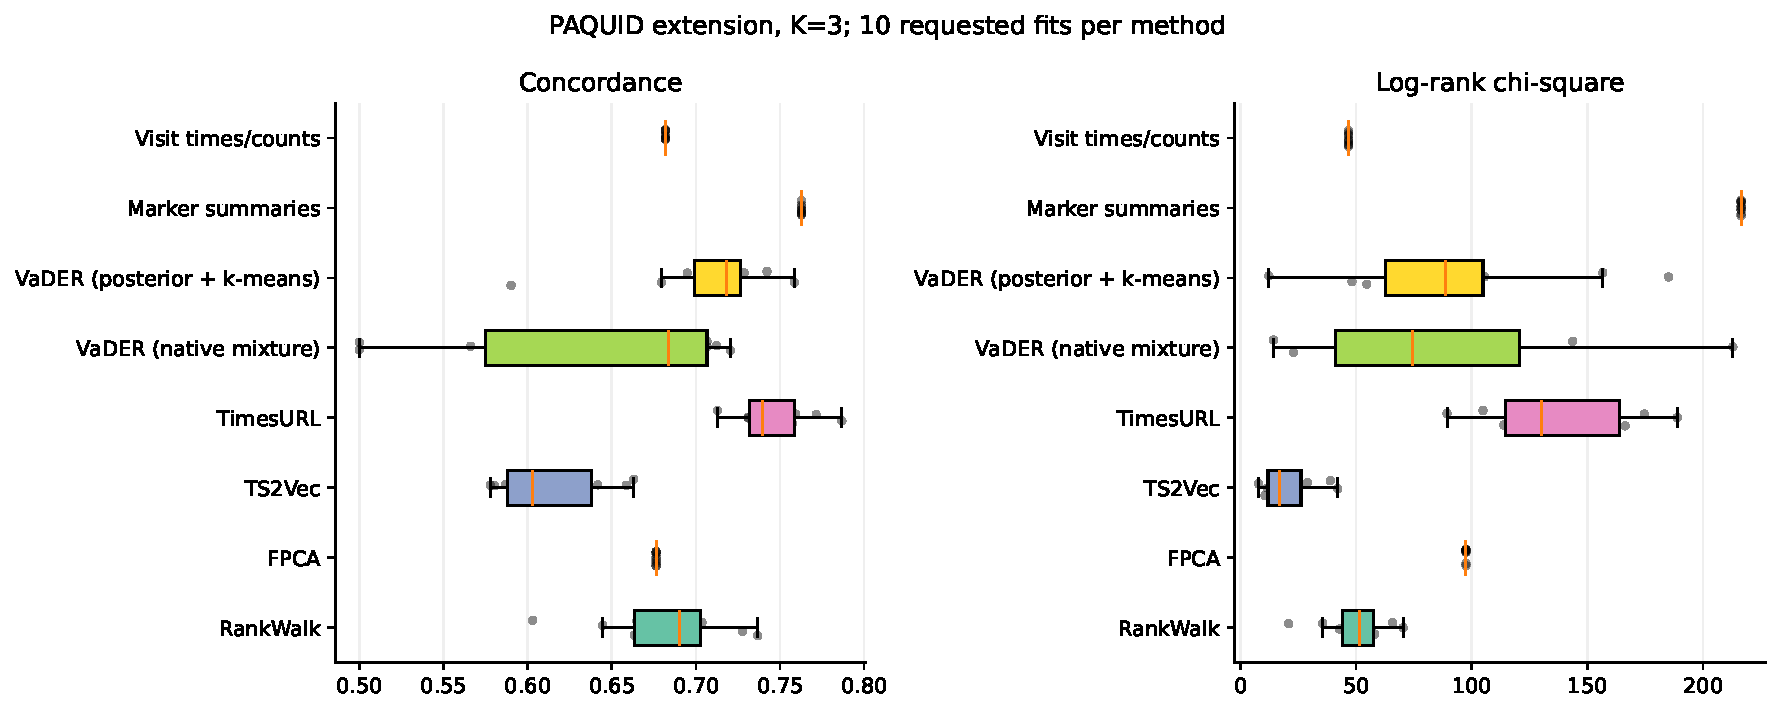
\includegraphics[width=\linewidth]{extension_PAQUID.pdf}\caption{PAQUID final extension distributions. Nine native VaDER successes are shown for RENAL and HEART. The PAQUID endpoint is corrected; these are full-follow-up associations.}\end{figure}

\begin{figure}[htbp]\centering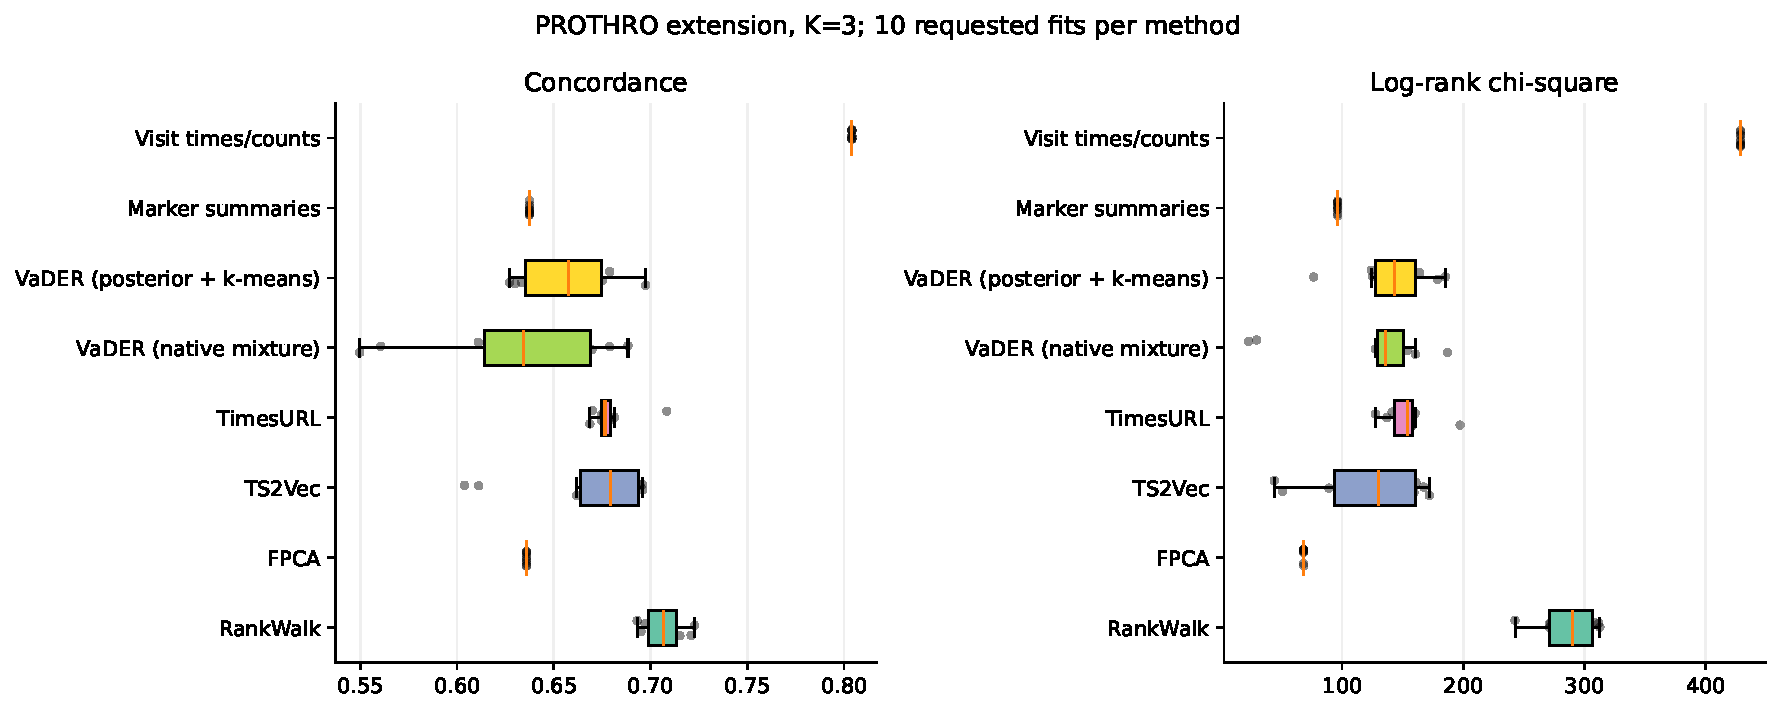
\includegraphics[width=\linewidth]{extension_PROTHRO.pdf}\caption{PROTHRO final extension distributions. Nine native VaDER successes are shown for RENAL and HEART. The PAQUID endpoint is corrected; these are full-follow-up associations.}\end{figure}

\begin{figure}[htbp]\centering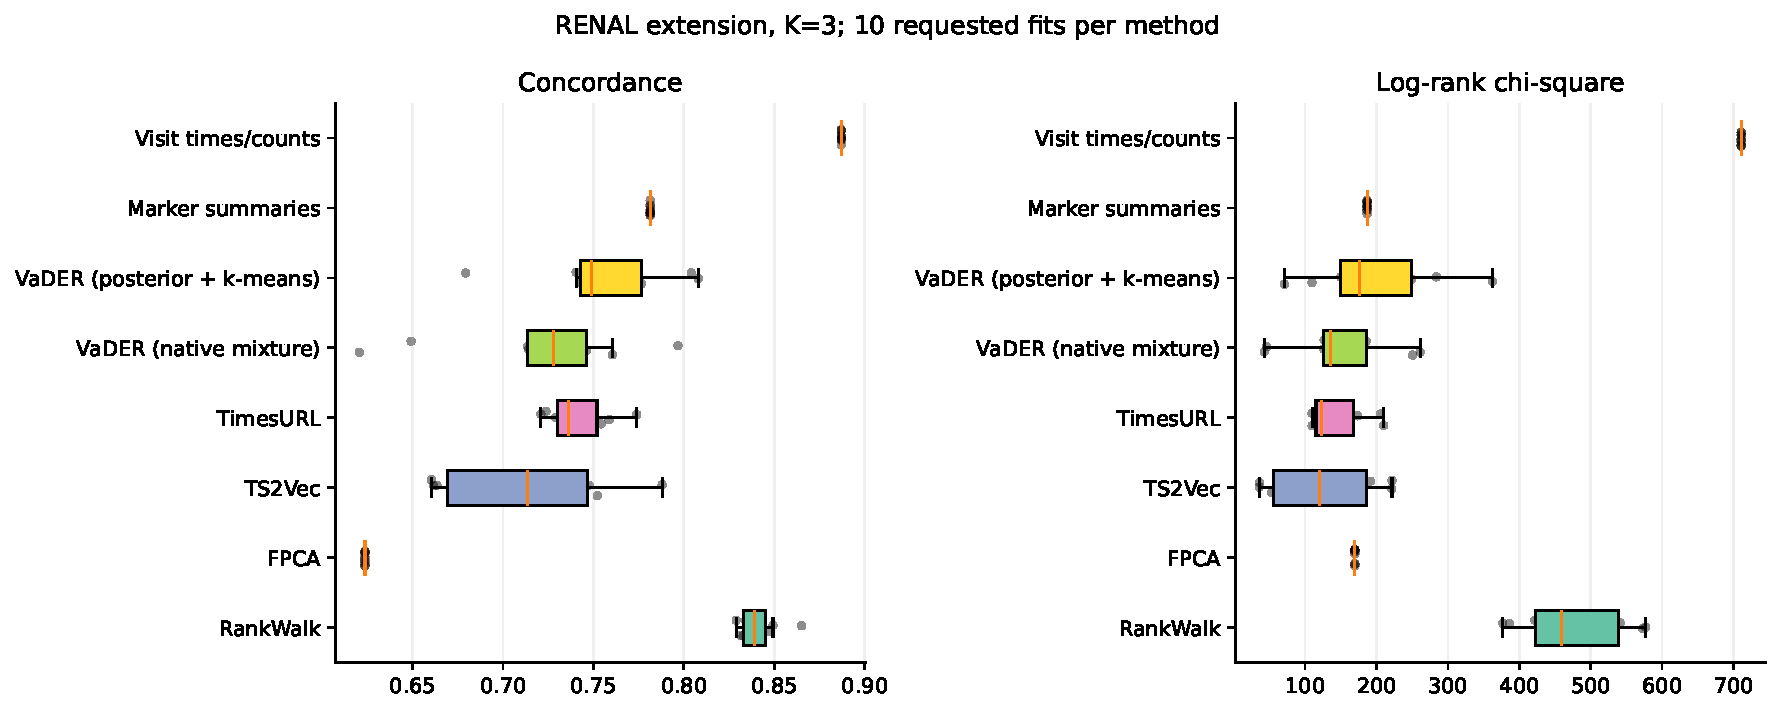
\includegraphics[width=\linewidth]{extension_RENAL.pdf}\caption{RENAL final extension distributions. Nine native VaDER successes are shown for RENAL and HEART. The PAQUID endpoint is corrected; these are full-follow-up associations.}\end{figure}

\begin{figure}[htbp]\centering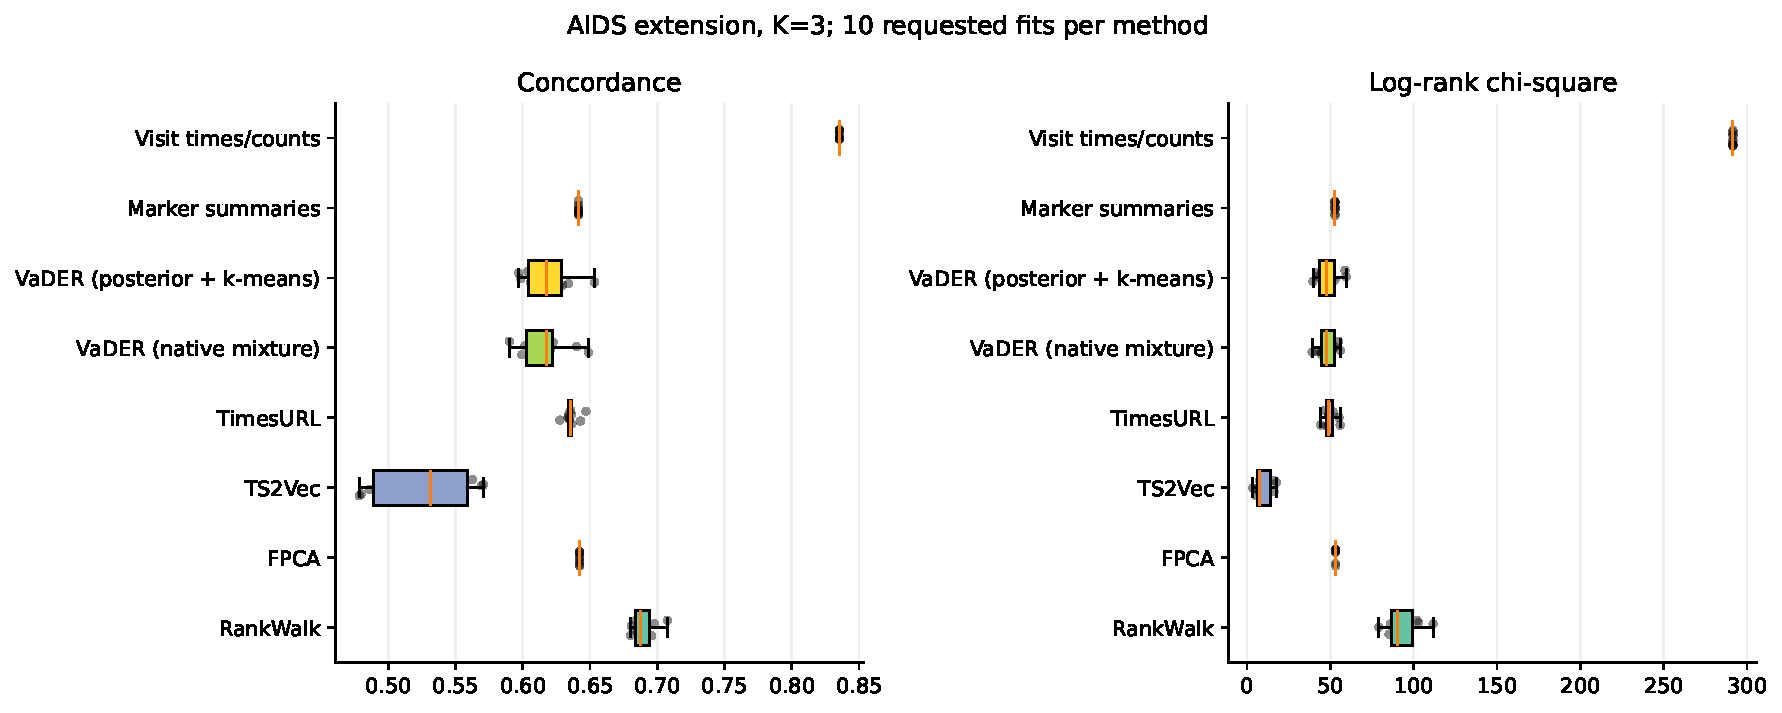
\includegraphics[width=\linewidth]{extension_AIDS.pdf}\caption{AIDS final extension distributions. Nine native VaDER successes are shown for RENAL and HEART. The PAQUID endpoint is corrected; these are full-follow-up associations.}\end{figure}

\begin{figure}[htbp]\centering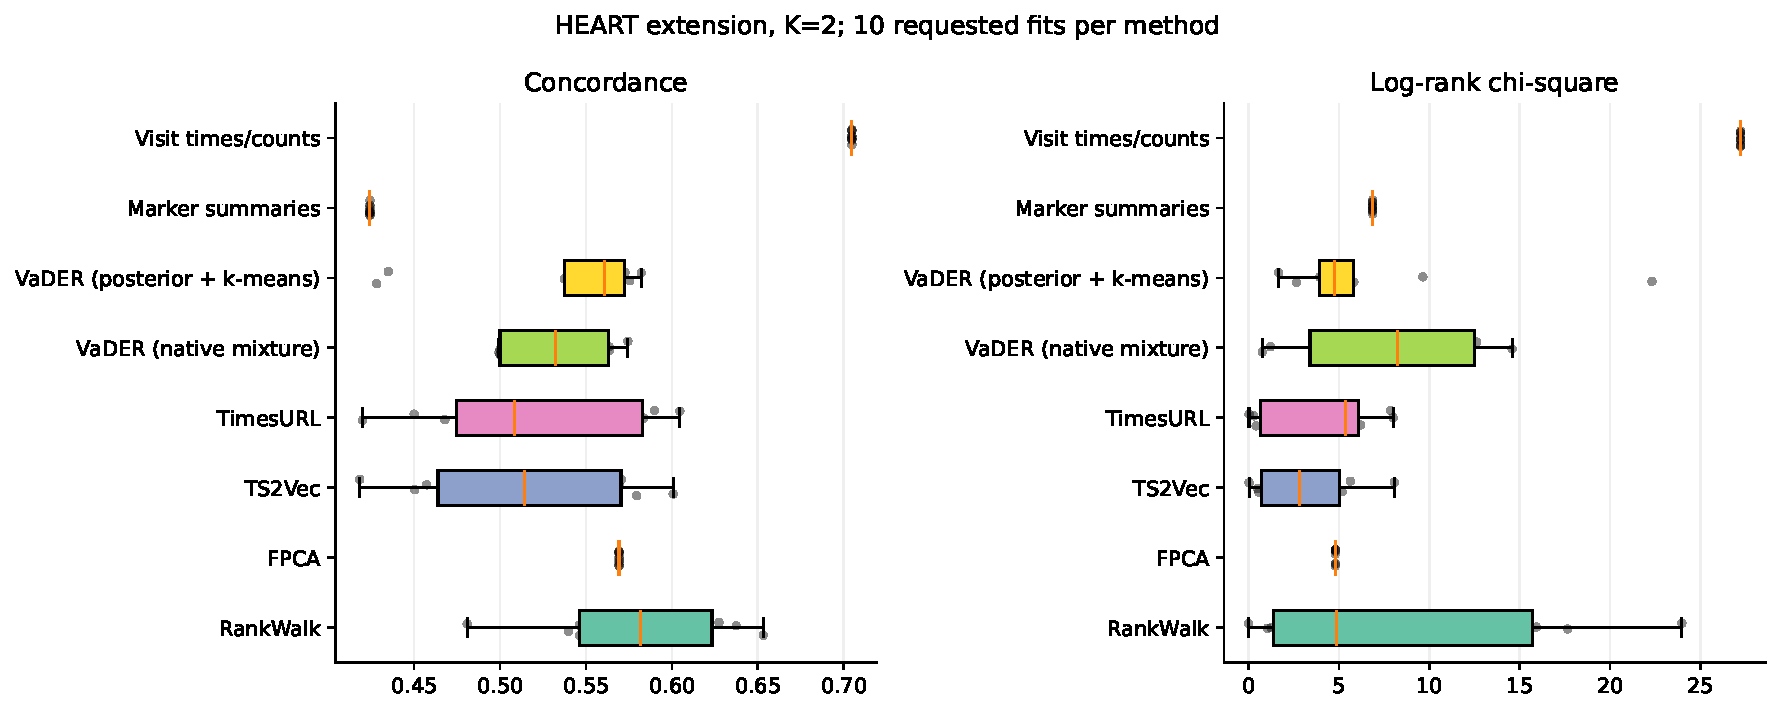
\includegraphics[width=\linewidth]{extension_HEART.pdf}\caption{HEART final extension distributions. Nine native VaDER successes are shown for RENAL and HEART. The PAQUID endpoint is corrected; these are full-follow-up associations.}\end{figure}

\clearpage\section{Clinical sensitivity checks}

\subsection{Saved-representation cluster-count sensitivity}

\begin{table}[htbp]
\centering\small
\caption{Saved-representation cluster-count sensitivity. Common Hmisc concordance and 100-start k-means are used; this is not identical to the native PAQUID Cox score.}
\begin{tabular}{lccccc}\toprule
Cohort & Method & $K$ & Fits & C-index & Log-rank $\chi^2$ \\ \midrule
AIDS & FPCA & 3 & 20 & $0.642 \pm 0.000$ & $53.09 \pm 0.00$ \\
AIDS & FPCA & 4 & 20 & $0.658 \pm 0.005$ & $63.24 \pm 1.28$ \\
AIDS & RankWalk & 3 & 20 & $0.689 \pm 0.006$ & $104.03 \pm 9.39$ \\
AIDS & RankWalk & 4 & 20 & $0.712 \pm 0.004$ & $113.41 \pm 4.66$ \\
HEART & FPCA & 2 & 20 & $0.569 \pm 0.000$ & $4.81 \pm 0.00$ \\
HEART & FPCA & 4 & 20 & $0.576 \pm 0.000$ & $7.78 \pm 0.00$ \\
HEART & RankWalk & 2 & 20 & $0.706 \pm 0.022$ & $54.16 \pm 8.41$ \\
HEART & RankWalk & 4 & 20 & $0.716 \pm 0.025$ & $51.92 \pm 6.61$ \\
PAQUID & FPCA & 3 & 30 & $0.659 \pm 0.000$ & $34.29 \pm 0.00$ \\
PAQUID & FPCA & 4 & 30 & $0.682 \pm 0.004$ & $43.62 \pm 0.81$ \\
PAQUID & RankWalk & 3 & 30 & $0.705 \pm 0.015$ & $40.20 \pm 5.05$ \\
PAQUID & RankWalk & 4 & 30 & $0.705 \pm 0.018$ & $38.27 \pm 6.17$ \\
PBC2 & FPCA & 3 & 20 & $0.760 \pm 0.000$ & $127.50 \pm 0.00$ \\
PBC2 & FPCA & 4 & 20 & $0.791 \pm 0.000$ & $216.28 \pm 0.00$ \\
PBC2 & RankWalk & 3 & 20 & $0.788 \pm 0.018$ & $240.79 \pm 26.95$ \\
PBC2 & RankWalk & 4 & 20 & $0.797 \pm 0.010$ & $254.82 \pm 23.25$ \\
\bottomrule\end{tabular}
\end{table}

\subsection{PAQUID onset-age correction on saved native representations}

\begin{table}[htbp]
\centering\small
\caption{PAQUID onset-age correction on saved native representations. Common Hmisc concordance and 100-start k-means are used; this is not identical to the native PAQUID Cox score.}
\begin{tabular}{lccccc}\toprule
Cohort & Method & $K$ & Fits & C-index & Log-rank $\chi^2$ \\ \midrule
PAQUID & FPCA & 3 & 30 & $0.676 \pm 0.000$ & $97.55 \pm 0.00$ \\
PAQUID & FPCA & 4 & 30 & $0.684 \pm 0.004$ & $107.31 \pm 1.43$ \\
PAQUID & RankWalk & 3 & 30 & $0.760 \pm 0.021$ & $108.06 \pm 14.52$ \\
PAQUID & RankWalk & 4 & 30 & $0.755 \pm 0.016$ & $107.48 \pm 9.44$ \\
\bottomrule\end{tabular}
\end{table}

The onset-corrected analysis of saved native PAQUID flattened representations and the newly trained mean-pooling extension are distinct experiments. Their scores should not be pooled or substituted for each other. Changing $K$ also changes log-rank degrees of freedom; larger raw chi-square alone is not a fair cross-$K$ selection criterion.

\clearpage\section{Failures, runtime, and limitations}

\begin{table}[htbp]
\centering\small
\caption{Documented numerical failures. Original seeds and model settings were retained on retry; no successful replacement seed was selected.}
\begin{tabular}{lcc}\toprule
Setting & VaDER success / attempted & Failure \\ \midrule
S2 regular & 49 / 50 & Singular covariance \\
RENAL extension & 9 / 10 & Mixture initialization covariance \\
HEART extension & 9 / 10 & Singular covariance \\
\bottomrule\end{tabular}
\end{table}

Failures remain part of the evaluation. Successful-fit summaries do not assign zero scores to failures and are therefore conditional on success. The failure audit and original error logs are bundled. All RankWalk fits completed.

Runtimes were collected during concurrent work on four CPU cores and under different algorithm-specific budgets. They are not controlled isolated speed comparisons. Sparse Jaccard and the Numba sampler were active for RankWalk; stochastic streams differ from the Torch backend, so identical learned partitions are not guaranteed. No new isolated old-versus-fast speedup factor is claimed here.

Clinical graph construction and representation learning are transductive over the observed cohort. Concordance risk ordering and categorical Cox fitting reuse outcome information for evaluation. Visit duration, density and eventual follow-up contribute substantial signal. A separate fixed-landmark design, appropriate censoring treatment and held-out patient evaluation are needed to assess prospective predictive value. Clinical uncertainty should additionally be assessed by patient resampling, rather than interpreting fit-to-fit SD as a confidence interval.

The competitors are selected established methods, not an exhaustive survey of every method available in 2026. Their fixed source budgets are not equal-FLOP budgets or a fully optimized performance frontier. New cohort selection and model comparisons are exploratory.

\section{Reproducibility package}
This source compiles without absolute workspace paths. Run \texttt{make} or execute \texttt{pdflatex report.tex} twice. The \texttt{figures/} directory includes vector PDF and PNG plots; \texttt{data/} includes all consolidated CSVs; \texttt{provenance/} includes source commits, environment versions, source portability patches and audits; \texttt{logs/} retains the three failure logs. Clinical CSVs contain derived subject-level analysis outputs; the original public cohort files are not redistributed in this package. This package contains generated outputs and report sources, not a replacement for the complete training environments.

\begin{thebibliography}{9}
\bibitem{rankwalk} Pfeifer, B. \emph{Contrastive Representation Learning of Longitudinal Disease Trajectories on Temporal Graphs}. arXiv:2607.25609, uploaded reference PDF, 2026.
\bibitem{ts2vec} Yue, Z., et al. \emph{TS2Vec: Towards Universal Representation of Time Series}. AAAI, 2022. Official implementation: \url{https://github.com/yuezhihan/ts2vec}.
\bibitem{timesurl} Liu, J. and Chen, S. \emph{TimesURL: Self-Supervised Contrastive Learning for Universal Time Series Representation Learning}. AAAI 38(12), 13918--13926, 2024. \url{https://github.com/Alrash/TimesURL}.
\bibitem{vader} de Jong, J., et al. VaDER, \emph{GigaScience}, 2019, doi:10.1093/gigascience/giz134. \url{https://github.com/johanndejong/VaDER}.
\bibitem{pace} Wang, J.-L., Chiou, J.-M. and M\"uller, H.-G. Functional Data Analysis. \emph{Annual Review of Statistics and Its Application}, 2016. Native \texttt{fdapace} package; exact version in provenance.
\end{thebibliography}
\appendix
\clearpage\section{Example simulated trajectories}


\begin{figure}[htbp]\centering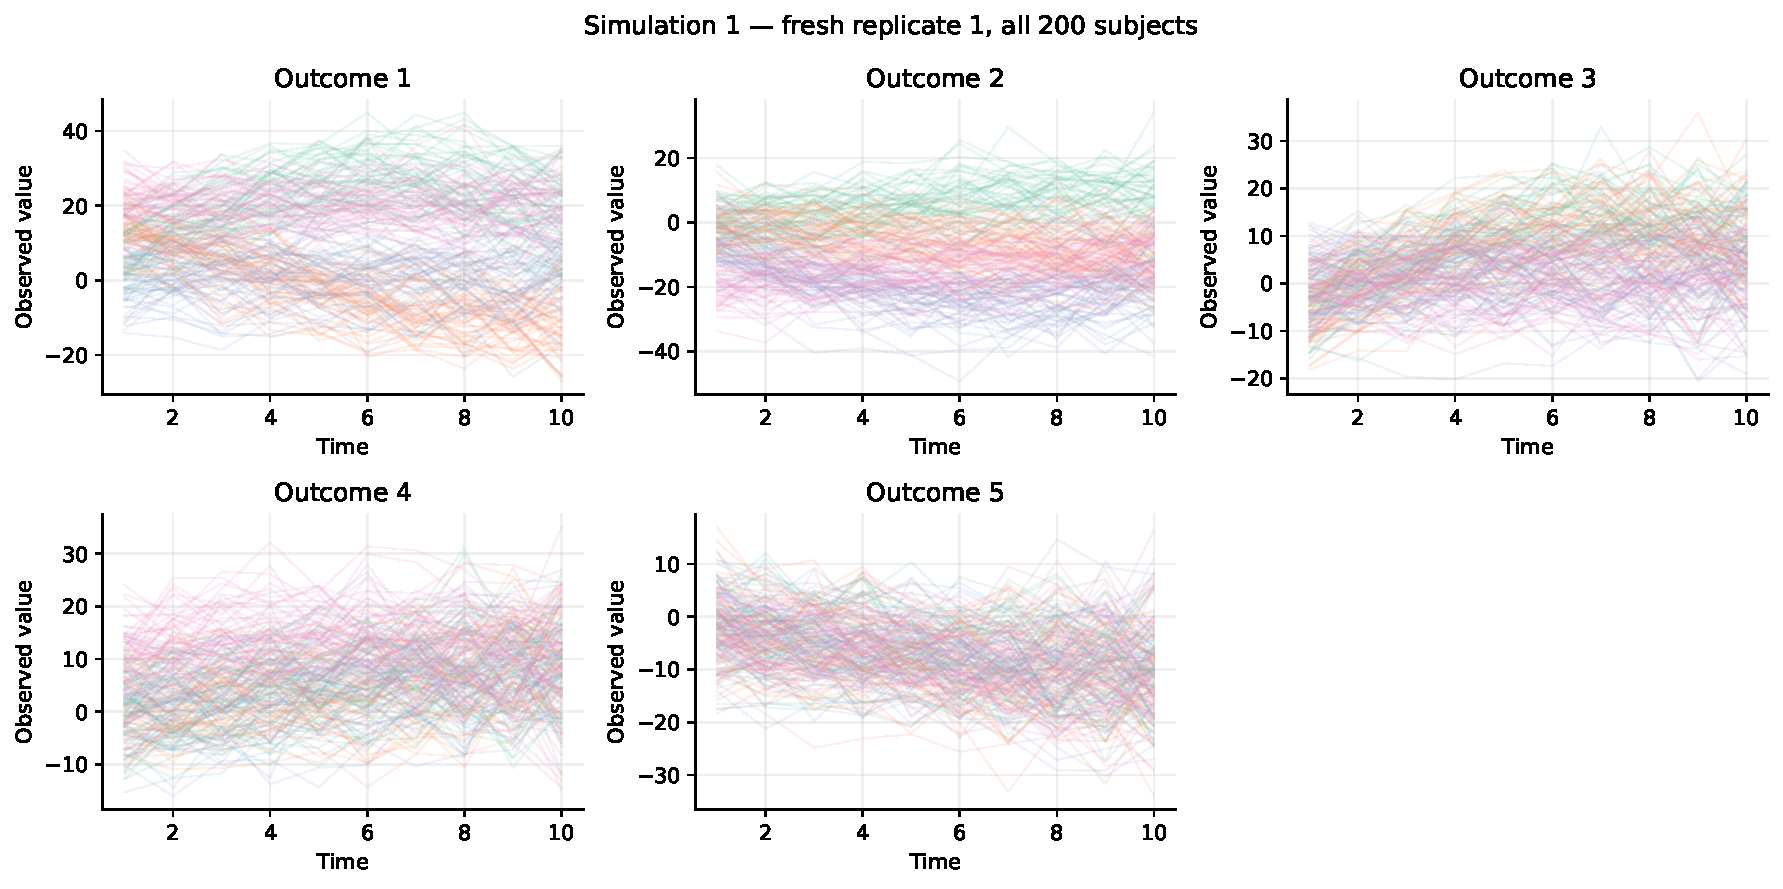
\includegraphics[width=\linewidth]{S1_clean_trajectories.pdf}\caption{Fresh Simulation 1 replicate 1: all 200 subjects, colored by ground-truth cluster.}\end{figure}

\begin{figure}[htbp]\centering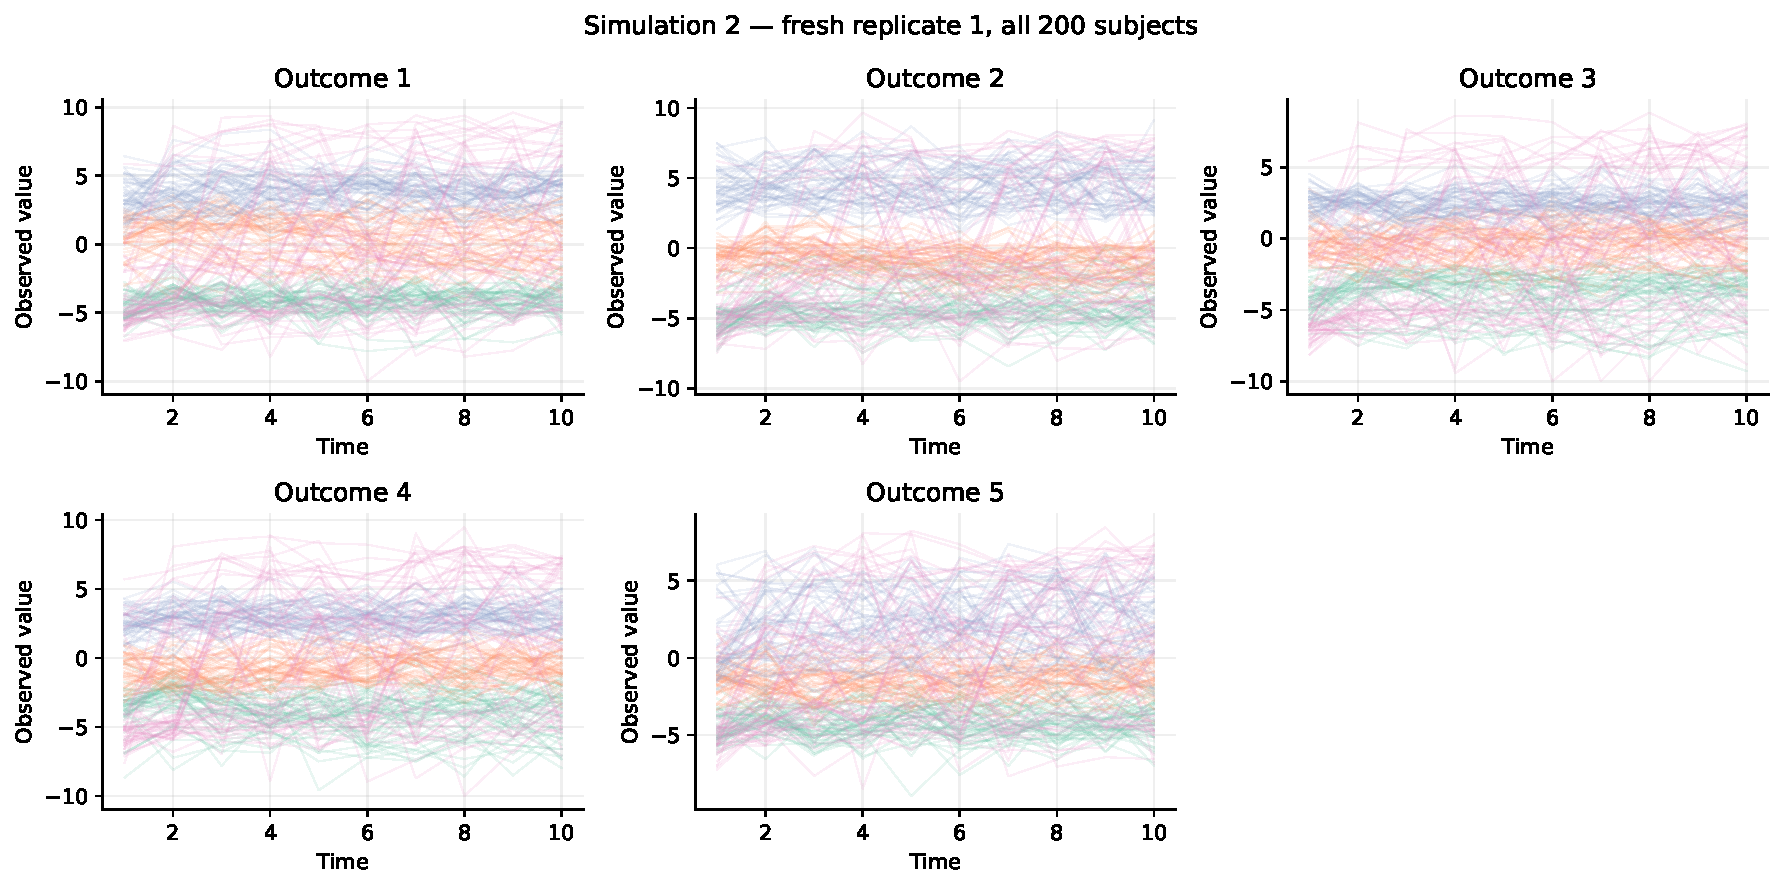
\includegraphics[width=\linewidth]{S2_regular_trajectories.pdf}\caption{Fresh Simulation 2 replicate 1: all 200 subjects, colored by ground-truth cluster.}\end{figure}

\clearpage\section{Source-input leakage diagnostics}

\begin{table}[htbp]
\centering\small
\caption{Source serialization includes unobserved simulator regime state. These are diagnostic reproduction results and are excluded from the observed-data competitor ranking.}
\begin{tabular}{lcc}\toprule
Method using source S2 inputs & Fits & ARI \\ \midrule
FPCA & 50 & $0.654 \pm 0.019$ \\
DTW & 50 & $0.849 \pm 0.068$ \\
kml3d & 50 & $0.363 \pm 0.087$ \\
TAPIO PC1 & 50 & $0.398 \pm 0.094$ \\
TAPIO weighted & 50 & $0.413 \pm 0.106$ \\
TS2Vec (source serialization) & 50 & $0.922 \pm 0.056$ \\
\bottomrule\end{tabular}
\end{table}

\begin{figure}[htbp]\centering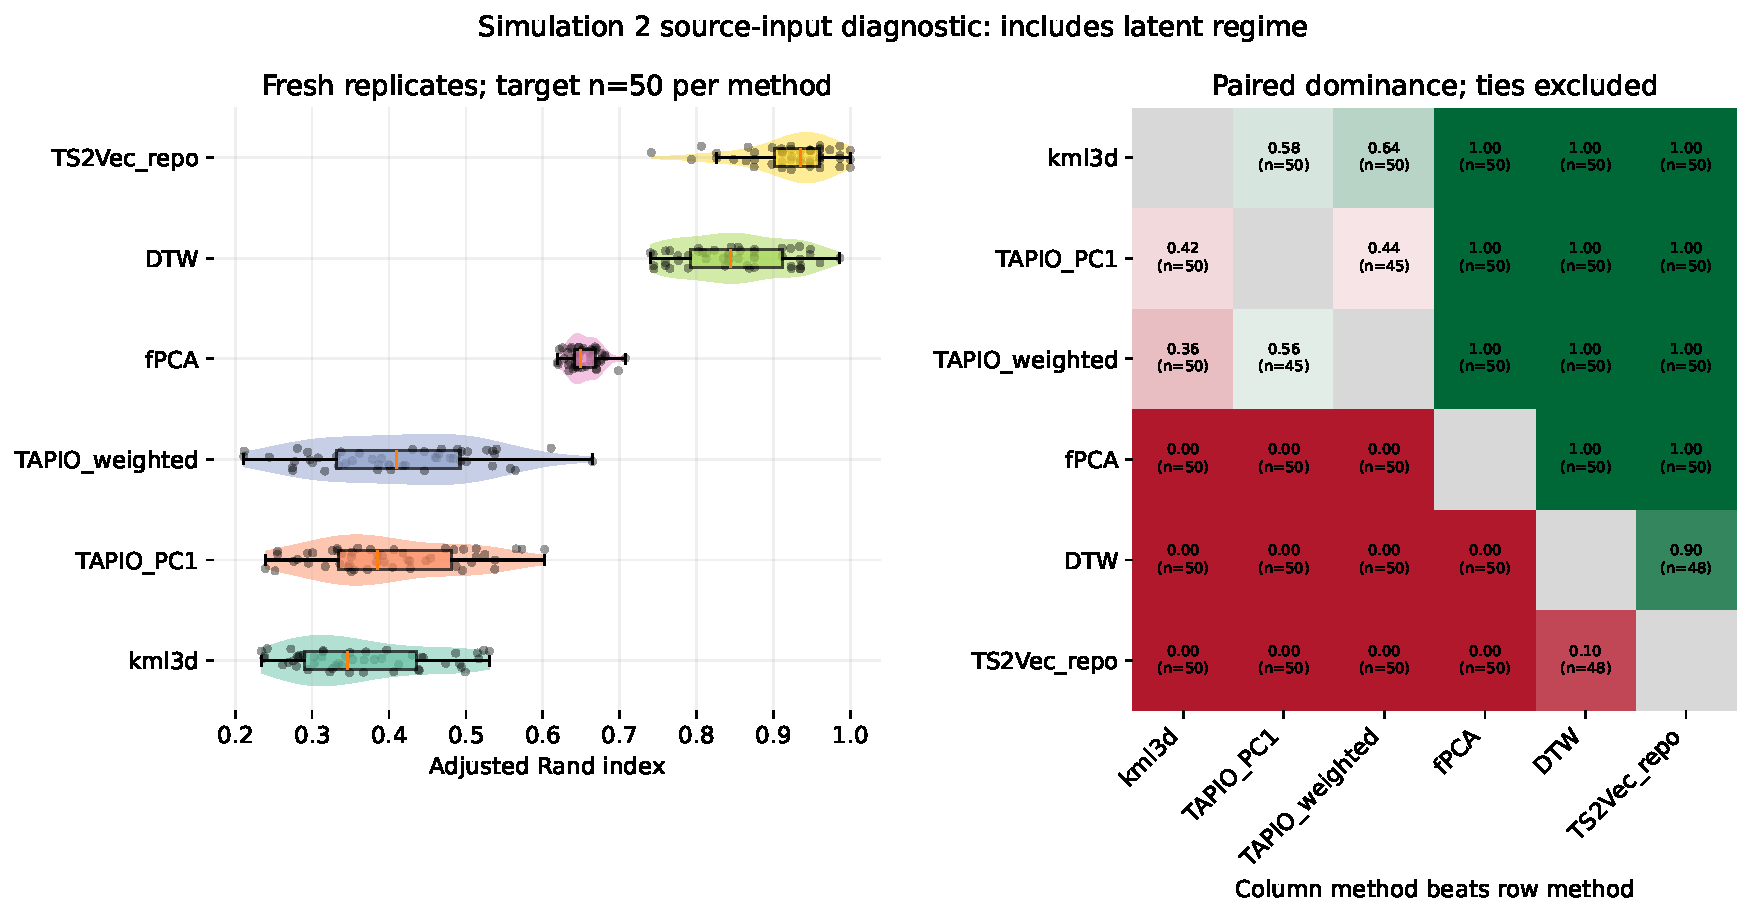
\includegraphics[width=\linewidth]{S2_regular_repo_latent_DIAGNOSTIC.pdf}\caption{Leaked-input source-script diagnostic only. These values must not be interpreted as observed-data comparator performance.}\end{figure}

\end{document}